\section{Event Loop and Network Layer}

\begin{frame}{Event Loop and Network Layer}{Event-Based Design}
  \begin{center}
    \begin{figure}
      \par\bigskip
      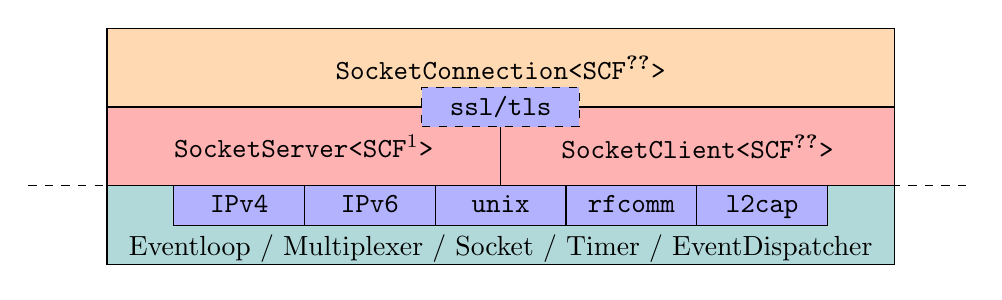
\begin{tikzpicture}
%%% Start Eventloop / Netzwerk
        \draw node[outer sep=0, draw, fill=teal!30, minimum width=10cm, minimum height=1cm] (em) {};
        \draw (em.center) node [anchor=north] {Eventloop / Multiplexer / Socket / Timer / EventDispatcher};
        \draw (em.north) node[xshift=-0.83cm, outer sep=0, inner sep=0, anchor=north east, draw, fill=blue!30, minimum height=0.5cm, minimum width=1.66cm] (ip6) {\texttt{\strut IPv6}};
        \draw (em.north) node[xshift=+0.83cm,outer sep=0, inner sep=0, anchor=north west, draw, fill=blue!30, minimum height=0.5cm, minimum width=1.66cm] (rfcomm) {\texttt{\strut rfcomm}};
        \draw (em.north) node[outer sep=0, inner sep=0, anchor=north, draw, fill=blue!30, minimum height=0.5cm, minimum width=1.66cm] (unix) {\texttt{\strut unix}};
        \draw (rfcomm.east) node[outer sep=0, inner sep=0, anchor=west, draw, fill=blue!30, minimum height=0.5cm, minimum width=1.66cm] (l2cap) {\texttt{\strut l2cap}};
        \draw (ip6.west) node[outer sep=0, inner sep=0, anchor=east, draw, fill=blue!30, minimum height=0.5cm, minimum width=1.66cm] (ip4) {\texttt{\strut IPv4}};
%%% End Eventloop / Netzwerk
%%$ Start draw dashed line above Eventloop-Layer
        \draw (em.north west) + (-1cm, 0) [dashed] -- ++(11cm, 0);
%%% End draw dashed line above Eventloop-Layer
%%% Start Lowlevel Server/Client
        \draw (em.north) node[anchor=south east, outer sep=0, draw, fill=red!30, minimum width=5cm, minimum height=1cm] (llst) {\texttt{SocketServer<SCF\footnote{\label{scf1}\texttt{SCF} \ldots \texttt{SocketContextFactory}}>}};
        \draw (em.north) node[anchor=south west, outer sep=0, draw, fill=red!30, minimum width=5cm, minimum height=1cm] (llct) {\texttt{SocketClient<SCF\textsuperscript{\ref{scf1}}>}};
%% End Lowlevel Server/Client
%% Start SocketConnection
        \draw (llst.north east) node[anchor=south, draw, fill=orange!30, inner sep=0, outer sep=0, minimum width=10cm, minimum height=1cm] {\texttt{SocketConnection<SCF\textsuperscript{\ref{scf1}}>}};
%% End SocketConnection
        \draw (llst.north east) node[outer sep=0, inner sep=0, anchor=center, draw, dashed, fill=blue!30, minimum width=2cm, minimum height=0.5cm] (ssl) {\texttt{ssl/tls}};
      \end{tikzpicture}
      \caption{The event loop and network layer in detail.}
    \end{figure}
  \end{center}
  Implementation details:
  \begin{itemize}
    \item \alert{Eventloop/Multiplexer/Timer/EventDispatcher}: Concrete classes, inheritance.
     \item \alert{Socket, SocketServer, -Client, -Connection and SSL/TLS}: Implemented as templates.
     \item \alert{IPv4, IPv6, unix, rfcomm, l2cap}: Implemented as a template class hierarchy.
  \end{itemize}
\end{frame}
